
The performance of the three classifiers -- linear discriminant, 
likelihood, and boosted decision tree -- 
are shown in Figs~\ref{fig:perf170mu}--\ref{fig:perf600mu}
for various Higgs mass points in terms of signal efficiency versus background rejection rate 
as the figure of merit.
The likelihood gives the best discrimination, therefore we use it 
for our analysis as will be described in detail in the next section.
%%%%%%%%%%%%%%%%%%%
\subsection{MVA performance: \texorpdfstring{$M_H$}{M(H)} = 170~GeV}
%%%%%%%%%%%%%%%%%%%
\begin{figure}[ht]
  \centering
  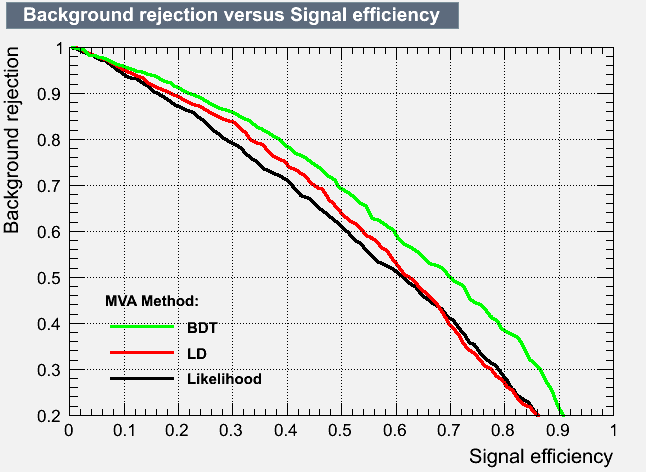
\includegraphics[width=0.48\textwidth]{figs/TMVA_170_nJ2_mu_rejBvsS}
  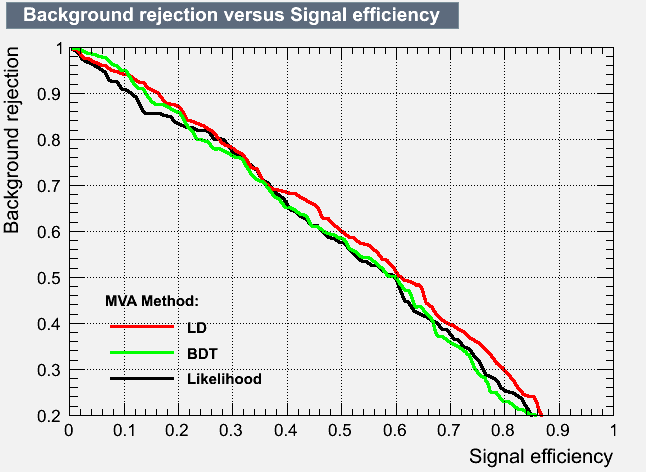
\includegraphics[width=0.48\textwidth]{figs/TMVA_170_nJ3_mu_rejBvsS}	
  \caption{\label{fig:perf170mu}Inputs to the multivariate discriminant for SM Higgs mass of 170~GeV for (a) 2-jet and (b) 3-jet $W\to\mu\nu$ category}
\end{figure}
%%%%%%%%%%%%%%%%%%%
\subsection{MVA performance: \texorpdfstring{$M_H$}{M(H)} = 180~GeV}
%%%%%%%%%%%%%%%%%%%
\begin{figure}[ht]
  \centering
  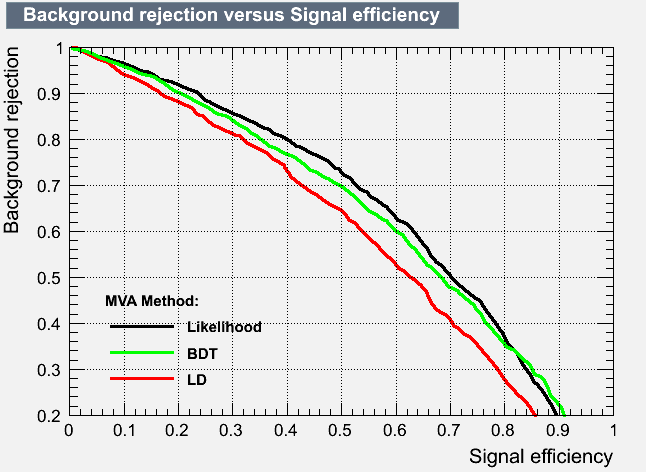
\includegraphics[width=0.48\textwidth]{figs/TMVA_180_nJ2_mu_rejBvsS}
  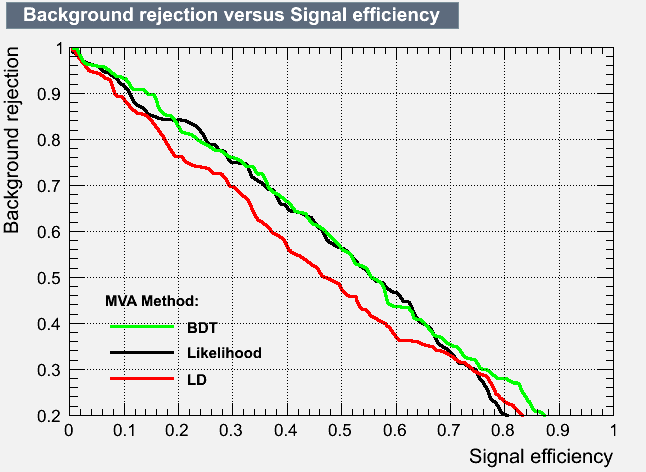
\includegraphics[width=0.48\textwidth]{figs/TMVA_180_nJ3_mu_rejBvsS}	
  \caption{\label{fig:perf180mu}Inputs to the multivariate discriminant for SM Higgs mass of 180~GeV for (a) 2-jet and (b) 3-jet $W\to\mu\nu$ category}
\end{figure}
%%%%%%%%%%%%%%%%%%%
\newpage
\subsection{MVA performance: \texorpdfstring{$M_H$}{M(H)} = 190~GeV}
%%%%%%%%%%%%%%%%%%%
\begin{figure}[ht]
  \centering
  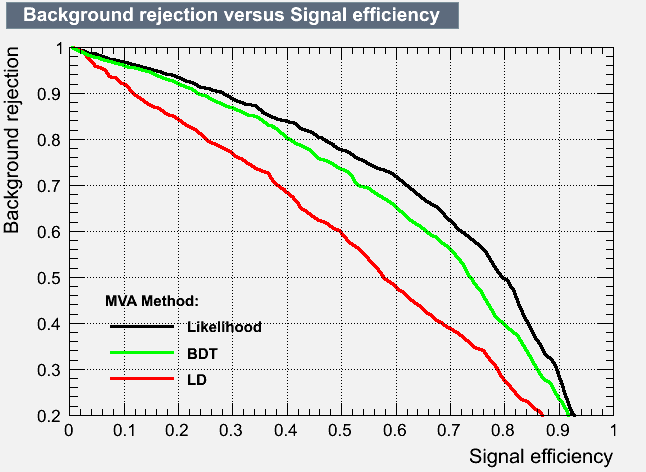
\includegraphics[width=0.48\textwidth]{figs/TMVA_190_nJ2_mu_rejBvsS}
  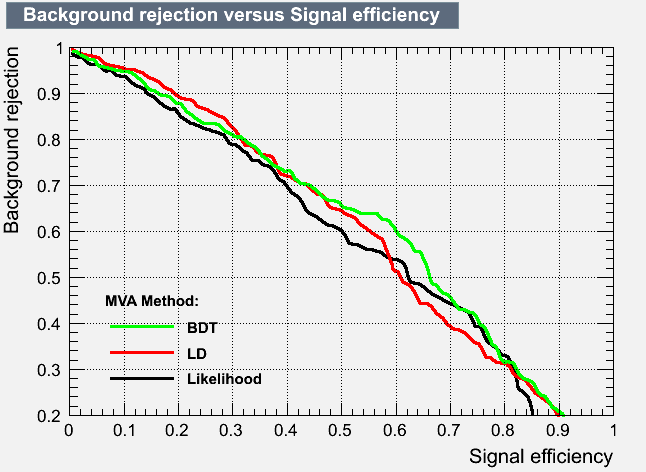
\includegraphics[width=0.48\textwidth]{figs/TMVA_190_nJ3_mu_rejBvsS}	
  \caption{\label{fig:perf190mu}Inputs to the multivariate discriminant for SM Higgs mass of 190~GeV for (a) 2-jet and (b) 3-jet $W\to\mu\nu$ category}
\end{figure}
%%%%%%%%%%%%%%%%%%%
\subsection{MVA performance: \texorpdfstring{$M_H$}{M(H)} = 200~GeV}
%%%%%%%%%%%%%%%%%%%
\begin{figure}[ht]
  \centering
  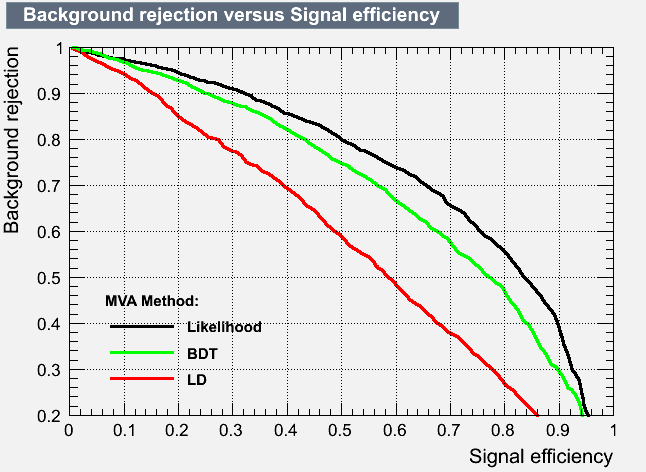
\includegraphics[width=0.48\textwidth]{figs/TMVA_200_nJ2_mu_rejBvsS}
  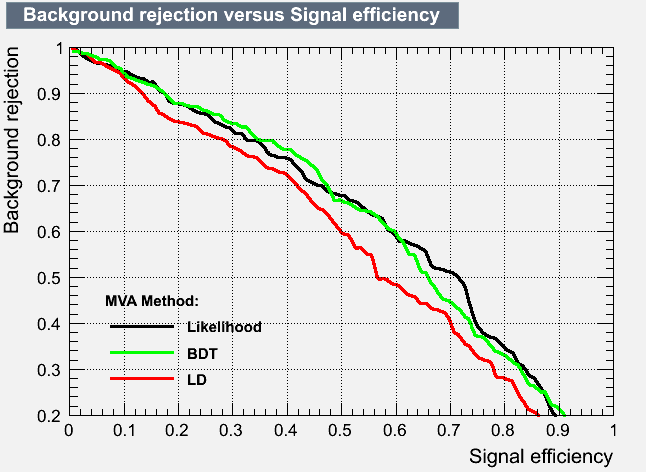
\includegraphics[width=0.48\textwidth]{figs/TMVA_200_nJ3_mu_rejBvsS}	
  \caption{\label{fig:perf200mu}Inputs to the multivariate discriminant for SM Higgs mass of 200~GeV for (a) 2-jet and (b) 3-jet $W\to\mu\nu$ category}
\end{figure}
%%%%%%%%%%%%%%%%%%%
\newpage
\subsection{MVA performance: \texorpdfstring{$M_H$}{M(H)} = 250~GeV}
%%%%%%%%%%%%%%%%%%%
\begin{figure}[ht]
  \centering
  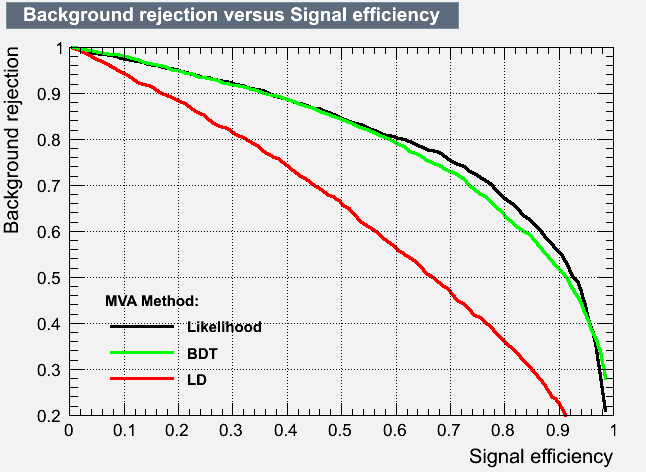
\includegraphics[width=0.48\textwidth]{figs/TMVA_250_nJ2_mu_rejBvsS}
  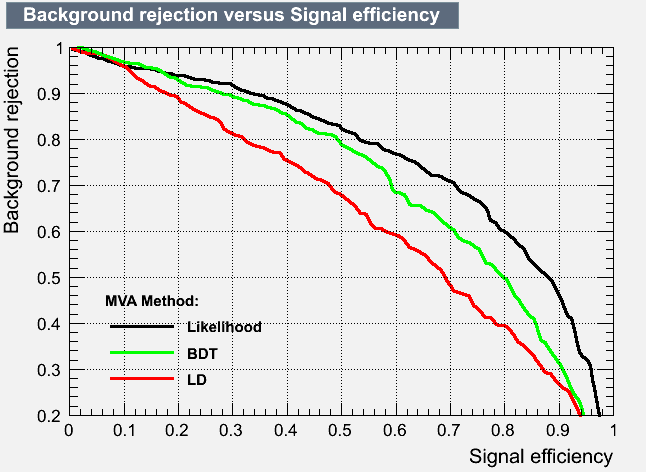
\includegraphics[width=0.48\textwidth]{figs/TMVA_250_nJ3_mu_rejBvsS}	
  \caption{\label{fig:perf250mu}Inputs to the multivariate discriminant for SM Higgs mass of 250~GeV for (a) 2-jet and (b) 3-jet $W\to\mu\nu$ category}
\end{figure}
%%%%%%%%%%%%%%%%%%%
\subsection{MVA performance: \texorpdfstring{$M_H$}{M(H)} = 300~GeV}
%%%%%%%%%%%%%%%%%%%
\begin{figure}[ht]
  \centering
  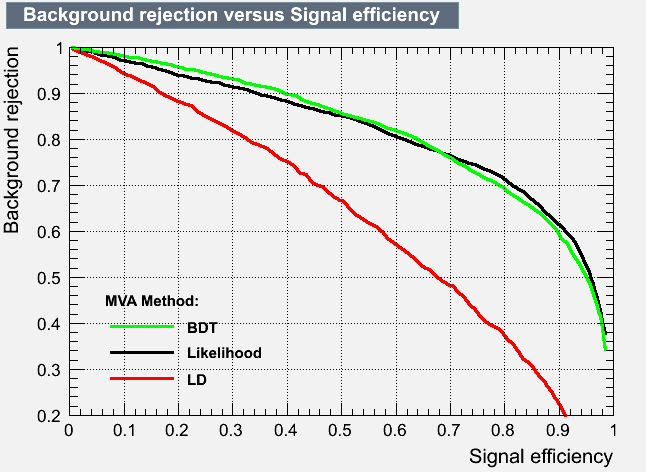
\includegraphics[width=0.48\textwidth]{figs/TMVA_300_nJ2_mu_rejBvsS}
  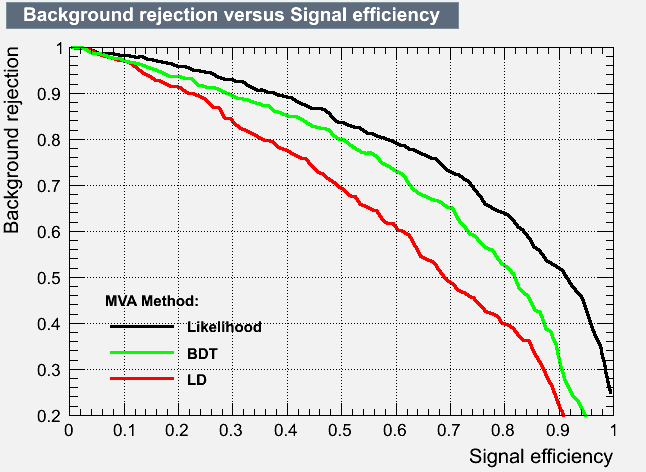
\includegraphics[width=0.48\textwidth]{figs/TMVA_300_nJ3_mu_rejBvsS}	
  \caption{\label{fig:perf300mu}Inputs to the multivariate discriminant for SM Higgs mass of 300~GeV for (a) 2-jet and (b) 3-jet $W\to\mu\nu$ category}
\end{figure}
%%%%%%%%%%%%%%%%%%%
\newpage
\subsection{MVA performance: \texorpdfstring{$M_H$}{M(H)} = 350~GeV}
%%%%%%%%%%%%%%%%%%%
\begin{figure}[ht]
  \centering
  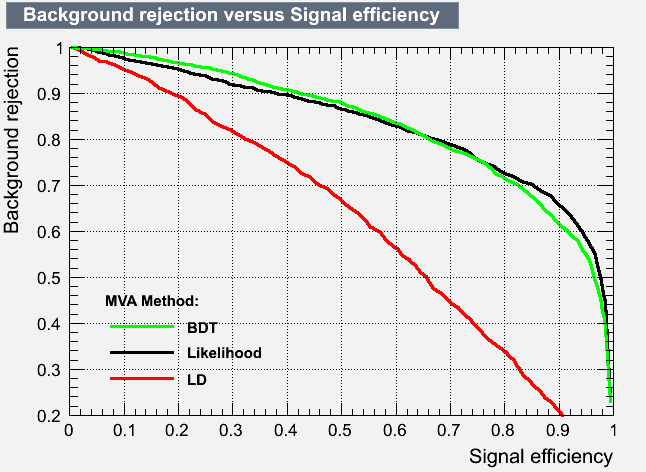
\includegraphics[width=0.48\textwidth]{figs/TMVA_350_nJ2_mu_rejBvsS}
  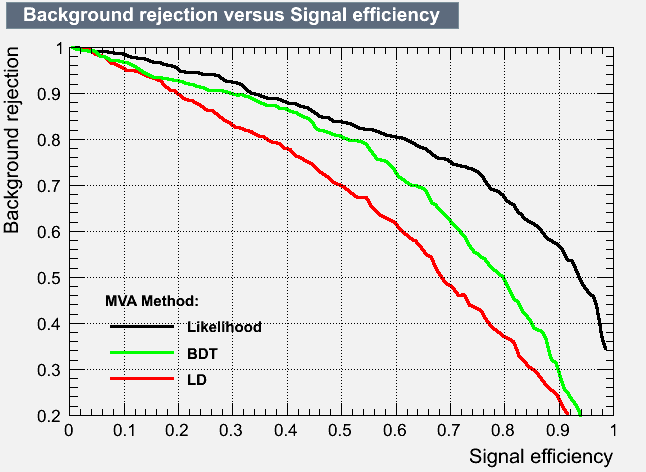
\includegraphics[width=0.48\textwidth]{figs/TMVA_350_nJ3_mu_rejBvsS}	
  \caption{\label{fig:perf350mu}Inputs to the multivariate discriminant for SM Higgs mass of 350~GeV for (a) 2-jet and (b) 3-jet $W\to\mu\nu$ category}
\end{figure}
%%%%%%%%%%%%%%%%%%%
\subsection{MVA performance: \texorpdfstring{$M_H$}{M(H)} = 400~GeV}
%%%%%%%%%%%%%%%%%%%
\begin{figure}[ht]
  \centering
  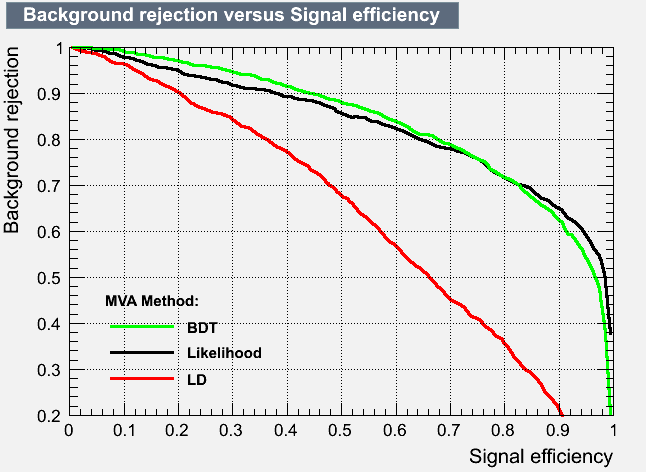
\includegraphics[width=0.48\textwidth]{figs/TMVA_400_nJ2_mu_rejBvsS}
  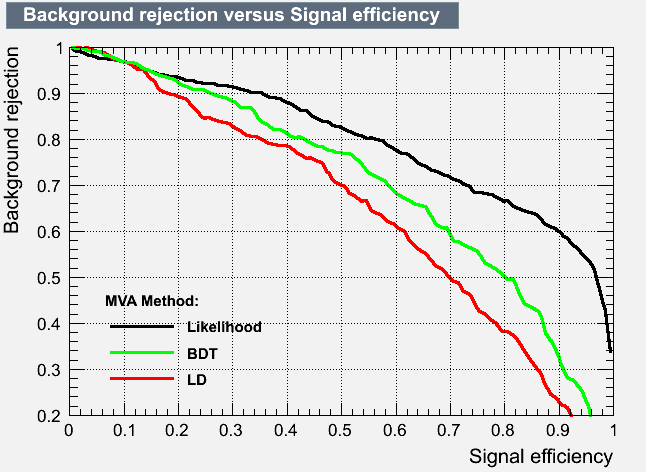
\includegraphics[width=0.48\textwidth]{figs/TMVA_400_nJ3_mu_rejBvsS}	
  \caption{\label{fig:perf400mu}Inputs to the multivariate discriminant for SM Higgs mass of 400~GeV for (a) 2-jet and (b) 3-jet $W\to\mu\nu$ category}
\end{figure}
%%%%%%%%%%%%%%%%%%%
\newpage
\subsection{MVA performance: \texorpdfstring{$M_H$}{M(H)} = 450~GeV}
%%%%%%%%%%%%%%%%%%%
\begin{figure}[ht]
  \centering
  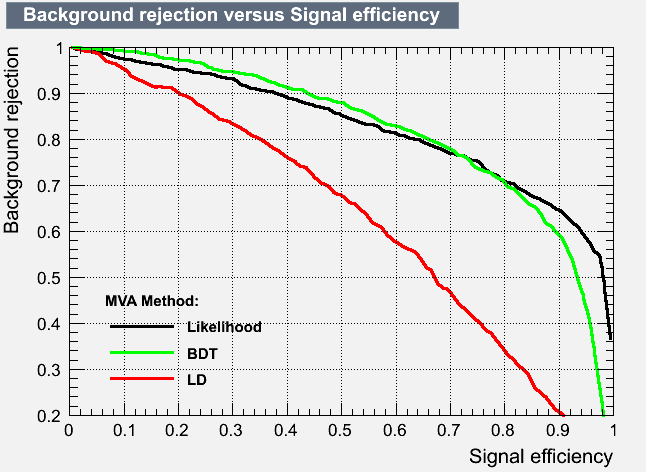
\includegraphics[width=0.48\textwidth]{figs/TMVA_450_nJ2_mu_rejBvsS}
  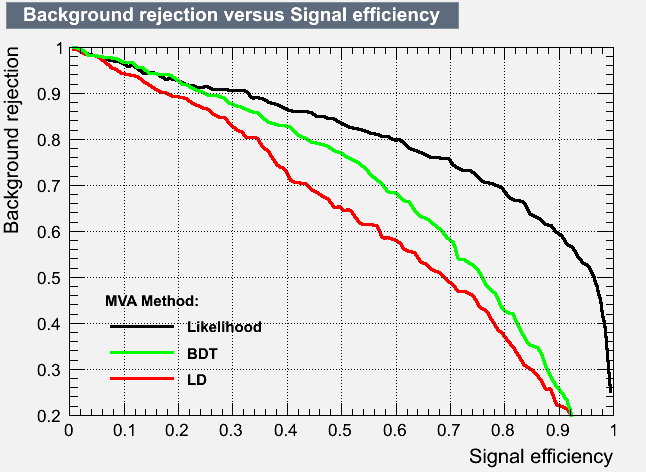
\includegraphics[width=0.48\textwidth]{figs/TMVA_450_nJ3_mu_rejBvsS}	
  \caption{\label{fig:perf450mu}Inputs to the multivariate discriminant for SM Higgs mass of 450~GeV for (a) 2-jet and (b) 3-jet $W\to\mu\nu$ category}
\end{figure}
%%%%%%%%%%%%%%%%%%%
\subsection{MVA performance: \texorpdfstring{$M_H$}{M(H)} = 500~GeV}
%%%%%%%%%%%%%%%%%%%
\begin{figure}[ht]
  \centering
  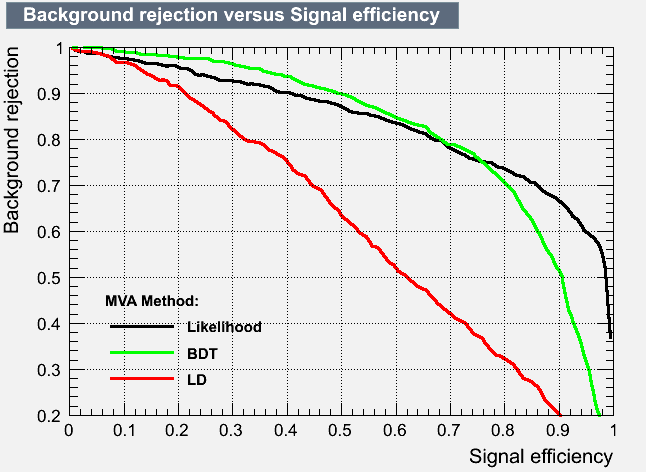
\includegraphics[width=0.48\textwidth]{figs/TMVA_500_nJ2_mu_rejBvsS}
  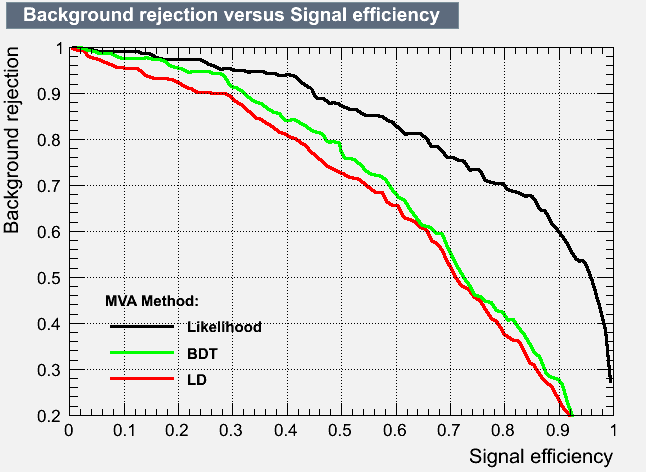
\includegraphics[width=0.48\textwidth]{figs/TMVA_500_nJ3_mu_rejBvsS}	
  \caption{\label{fig:perf500mu}Inputs to the multivariate discriminant for SM Higgs mass of 500~GeV for (a) 2-jet and (b) 3-jet $W\to\mu\nu$ category}
\end{figure}
%%%%%%%%%%%%%%%%%%%
\newpage
\subsection{MVA performance: \texorpdfstring{$M_H$}{M(H)} = 550~GeV}
%%%%%%%%%%%%%%%%%%%
\begin{figure}[ht]
  \centering
  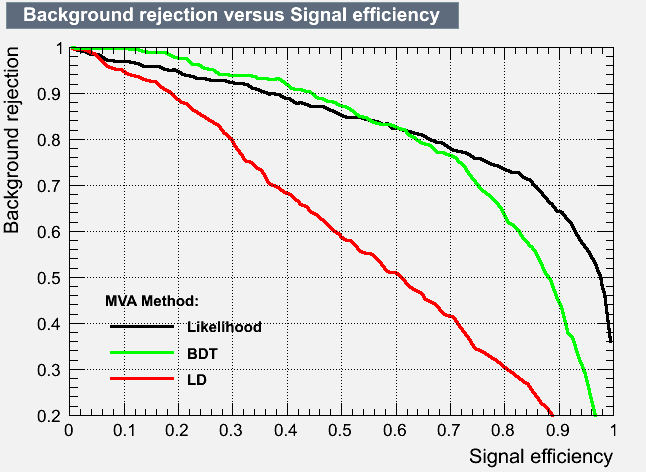
\includegraphics[width=0.48\textwidth]{figs/TMVA_550_nJ2_mu_rejBvsS}
  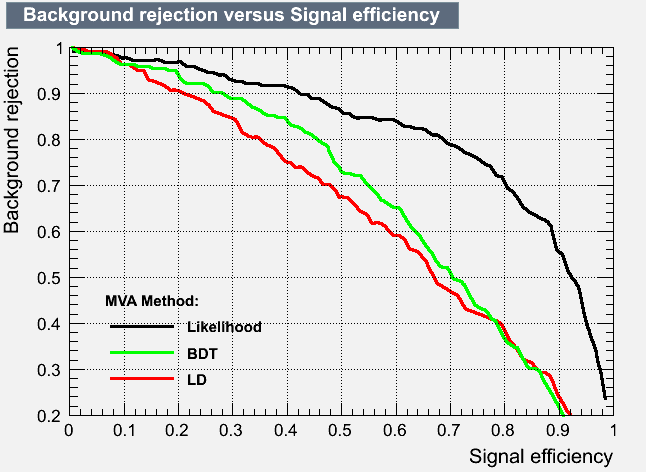
\includegraphics[width=0.48\textwidth]{figs/TMVA_550_nJ3_mu_rejBvsS}	
  \caption{\label{fig:perf550mu}Inputs to the multivariate discriminant for SM Higgs mass of 550~GeV for (a) 2-jet and (b) 3-jet $W\to\mu\nu$ category}
\end{figure}
%%%%%%%%%%%%%%%%%%%
\subsection{MVA performance: \texorpdfstring{$M_H$}{M(H)} = 600~GeV}
%%%%%%%%%%%%%%%%%%%
\begin{figure}[ht]
  \centering
  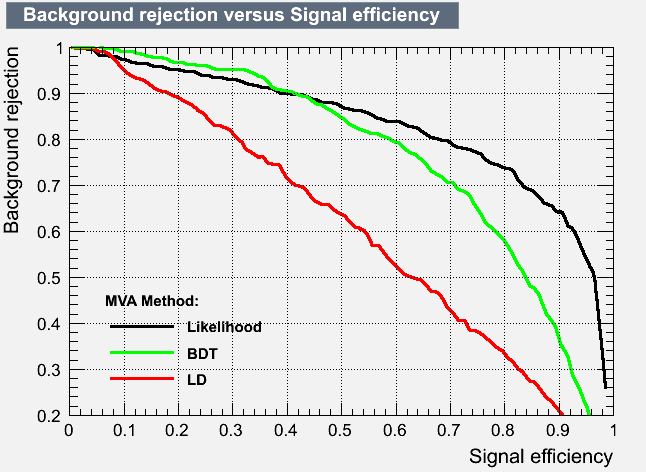
\includegraphics[width=0.48\textwidth]{figs/TMVA_600_nJ2_mu_rejBvsS}
  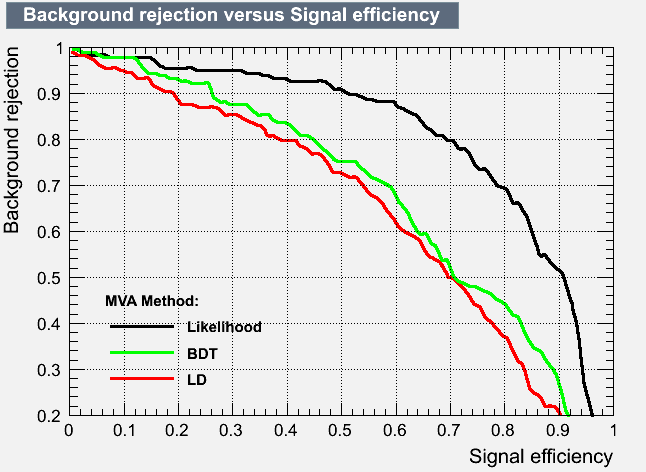
\includegraphics[width=0.48\textwidth]{figs/TMVA_600_nJ3_mu_rejBvsS}	
  \caption{\label{fig:perf600mu}Inputs to the multivariate discriminant for SM Higgs mass of 600~GeV for (a) 2-jet and (b) 3-jet $W\to\mu\nu$ category}
\end{figure}
%%%%%%%%%%%%%%%%%%%
